% ===========================================================================
% Problem formulation and package interface
% ===========================================================================

\begin{figure}[t]
    \centering
    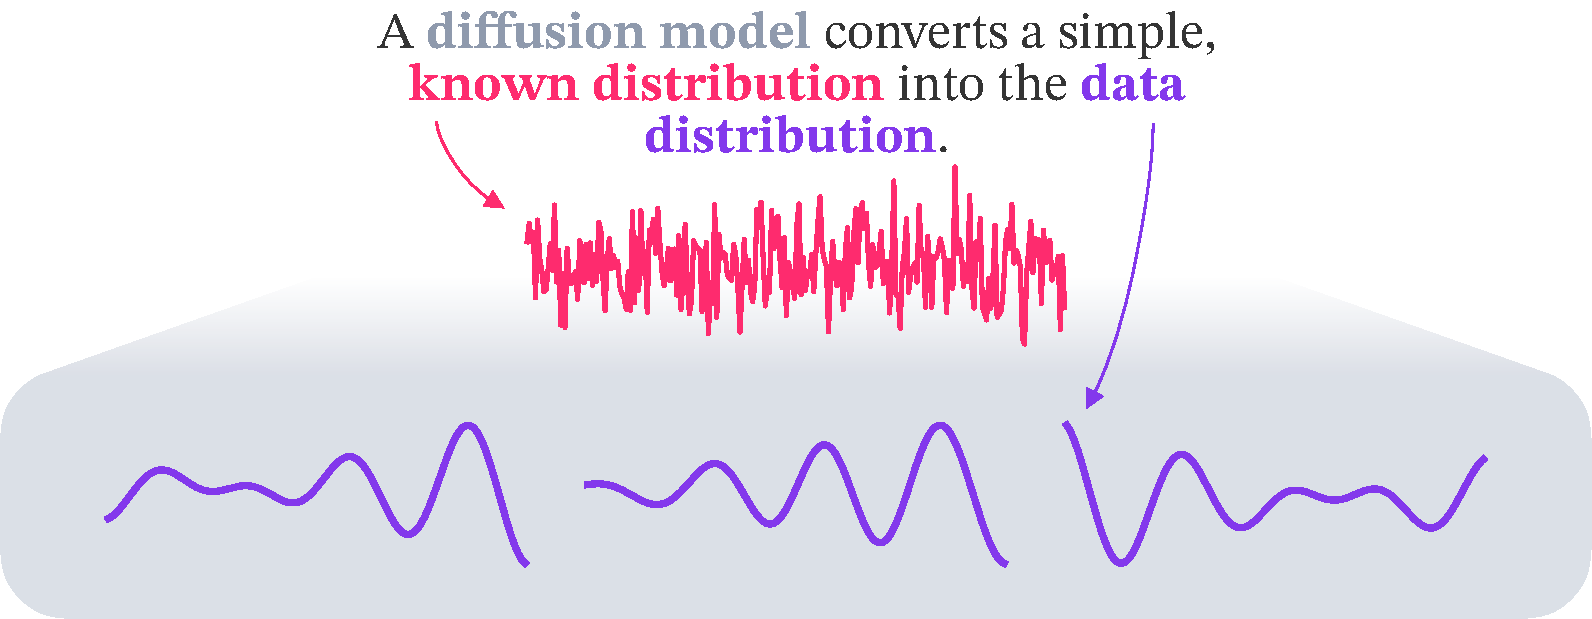
\includegraphics[width=0.8\textwidth]{diffusion_highlevel.pdf}
    \caption{Conditional diffusion model for stochastic trajectories. Training
    samples a clean trajectory, adds Gaussian noise at a selected diffusion
    level, and trains the denoiser to predict the added noise. Generation starts
    from Gaussian noise and applies the trained denoiser repeatedly to obtain a
    trajectory conditioned on $\mathbf{c}$. The diffusion index $k$ is distinct
    from the physical-time coordinate of the trajectory.}
    \label{fig:diffusion_highlevel}
\end{figure}

\section{Problem formulation}
\label{sec:physical_problem}
\subsection{Statement of the physical problem}

Consider a stochastic dynamical system with state $\mathbf{q}(t)\in\mathbb{R}^m$ governed by
\begin{equation}
    \mathrm{d}q_i
    =
    f_i(\mathbf{q},t;\boldsymbol{\lambda})\,\mathrm{d}t
    +
    \sum_{j=1}^{m_W}
    G_{ij}(\mathbf{q},t;\boldsymbol{\lambda})\,\mathrm{d}W_j,
    \qquad
    i=1,\ldots,m ,
    \label{eq:generic_sde_component}
\end{equation}
or, in vector form, $\mathrm{d}\mathbf{q}=\mathbf{f}(\mathbf{q},t;\boldsymbol{\lambda})\,\mathrm{d}t+\mathbf{G}(\mathbf{q},t;\boldsymbol{\lambda})\,\mathrm{d}\mathbf{W}.$
Here $\mathbf{f}$ is the drift, $\boldsymbol{\lambda}$ denotes physical parameters, $\mathbf{G}\in\mathbb{R}^{m\times m_W}$ is the diffusion matrix, and $\mathbf{W}(t)\in\mathbb{R}^{m_W}$ contains $m_W$ independent Wiener processes. State-independent $\mathbf{G}$ gives additive noise and state-dependent $\mathbf{G}$ gives multiplicative noise. The examples in this paper use additive noise. Coloured noise can be included by augmenting the state with an additional stochastic variable, as in the Duffing oscillator of Section~\ref{ssec:duffing}.

The package does not attempt to infer $\mathbf{f}$ or $\mathbf{G}$ (which is a divergence from e.g., a neural SDE). Instead, it learns the distribution of sampled trajectories produced by the stochastic system. The generated quantity is an approximation of a continuous trajectory $q(t)$. Sampling it at $N_T$ physical-time points gives the vector representation $\mathbf{q}^{(s)} = \left( q^{(s)}_0,\ldots,q^{(s)}_{N_T-1} \right) \in\mathbb{R}^{N_T}$, where $s=1,\ldots,N_S$, for an ensemble of $N_S$ realisations.

Each trajectory may also be associated with a conditioning vector $\mathbf{c}^{(s)}\in\mathbb{R}^{N_T}.$ The conditioning vector has the same length as the trajectory because it is supplied to the denoiser alongside the trajectory. It may represent a constant physical parameter, initial conditions stored in its leading entries and padded with zeros, or a time-dependent driving signal. If no physical conditioning is required, an empty conditioning vector can be used.

The physical system therefore defines a conditional trajectory distribution $\mathbf{q}\sim p_{\mathrm{data}}(\mathbf{q}\mid\mathbf{c}).$ The model learns $p_\phi(\mathbf{q}\mid\mathbf{c}) \approx p_{\mathrm{data}}(\mathbf{q}\mid\mathbf{c}),$ where $\phi$ denotes the trainable network parameters.

\subsection{Minimal package interface}
Training data are stored as a PyTorch dataset containing trajectory--condition pairs:

\begin{pythonlisting}
from torch.utils.data import TensorDataset

train_dataset = TensorDataset(
    trajectories,
    conditioning,
)
\end{pythonlisting}

We observe more reliable training and inference when trajectories and conditioning variables are standardised. The library provides the corresponding standardisation and inverse-standardisation utilities.

The complete model interface is

\begin{pythonlisting}
from diffusionsde import DDPM

model = DDPM() # assuming default parameters are used
history = model.fit(train_dataset)
samples = model.generate(conditioning)
\end{pythonlisting}

The remainder of this section is structured around these two operations. In \texttt{model.fit()}, Gaussian noise is added to a clean trajectory and the network learns to predict that noise from the corrupted trajectory, its diffusion index, and the condition. In \texttt{model.generate()}, the trained network is used repeatedly to transform Gaussian noise into a clean trajectory that looks similar to the training data.


\subsection{Training with \texttt{model.fit}}
\label{ssec:fit}

\subsubsection{Forward diffusion}

Diffusion introduces an artificial index $k$ that is distinct from physical time $t$. Where appropriate, we will refer to $k$ as the `algorithmic time'. Let $N_K$ be the number of diffusion steps, with $k=0$ denoting clean data. At each step, $\beta_k$ specifies the variance of the Gaussian noise introduced by that step. It is useful to define the related quantities $\alpha_k = 1-\beta_k$,  $\alphabar_k= \prod_{\ell=1}^{k}\alpha_\ell,$ and $\alphabar_0=1,$ where $\alpha_k$ is the fraction of signal variance retained in one forward step, while $\alphabar_k$ is the corresponding fraction retained after $k$ steps. Consequently, $\sqrt{\alphabar_k}$ determines the contribution of the original trajectory after $k$ steps and $1-\alphabar_k$ gives the accumulated noise variance.

The implementation uses a literature-standard linear schedule
\begin{equation}
    \beta_k
    =
    \beta_1
    +
    \frac{k-1}{N_K-1}
    \left(
        \beta_{N_K}-\beta_1
    \right),
    \qquad
    k=1,\ldots,N_K,
    \label{eq:beta_schedule}
\end{equation}
where
$0<\beta_1\leq\beta_{N_K}<1$. The forward transition is
\begin{equation}
    \mathbf{q}_k
    =
    \sqrt{\alpha_k}\,\mathbf{q}_{k-1}
    +
    \sqrt{\beta_k}\,\boldsymbol{\varepsilon}_k,
    \qquad
    \boldsymbol{\varepsilon}_k
    \sim
    \Normal(\mathbf{0},\mathsf{I}).
    \label{eq:forward_step}
\end{equation}
Successive steps reduce the contribution from the original trajectory and increase the Gaussian component.

Because the forward process is Gaussian, its marginal distribution is known analytically:
\begin{equation}
    p_{\mathrm{fwd}}
    (\mathbf{q}_k\mid\mathbf{q}_0)
    =
    \Normal\!\left(
        \mathbf{q}_k;
        \sqrt{\alphabar_k}\,\mathbf{q}_0,
        (1-\alphabar_k)\mathsf{I}
    \right).
    \label{eq:forward_marginal_density}
\end{equation}
A sample at any diffusion level can therefore be obtained directly as
\begin{equation}
    \mathbf{q}_k
    =
    \sqrt{\alphabar_k}\,\mathbf{q}_0
    +
    \sqrt{1-\alphabar_k}\,
    \boldsymbol{\varepsilon},
    \qquad
    \boldsymbol{\varepsilon}
    \sim
    \Normal(\mathbf{0},\mathsf{I}).
    \label{eq:forward_marginal}
\end{equation}
There is no need to evaluate the preceding $k-1$ forward steps during training.

\subsubsection{Noise-prediction objective}

For each training pair $(\mathbf{q}_0,\mathbf{c})$,
\texttt{model.fit} samples $ k\sim\mathrm{Unif}\{1,\ldots,N_K\}$, where $\boldsymbol{\varepsilon}\sim\Normal(\mathbf{0},\mathsf{I}),$ constructs $\mathbf{q}_k$ using Eq.~\eqref{eq:forward_marginal}, and passes $(\mathbf{q}_k,k,\mathbf{c})$ to the denoiser. The network output $\boldsymbol{\varepsilon}_\phi(\mathbf{q}_k,k,\mathbf{c}) $ is an estimate of the noise that was added at that denoising step.\footnote{The noise predictor is related to the score of the noisy trajectory distribution
\cite{hyvarinen2005score,vincent2011connection}. From
Eq.~\eqref{eq:forward_marginal_density},
\begin{equation}
    \nabla_{\mathbf{q}_k}
    \log
    p_{\mathrm{fwd}}
    (\mathbf{q}_k\mid\mathbf{q}_0)
    =
    -
    \frac{
        \boldsymbol{\varepsilon}
    }{
        \sqrt{1-\alphabar_k}
    }.
    \label{eq:conditional_score}
\end{equation}
The conditional distribution of noisy trajectories is
\begin{equation}
    p_k(\mathbf{q}_k\mid\mathbf{c})
    =
    \int
    p_{\mathrm{fwd}}
    (\mathbf{q}_k\mid\mathbf{q}_0)
    p_{\mathrm{data}}
    (\mathbf{q}_0\mid\mathbf{c})
    \,\mathrm{d}\mathbf{q}_0.
    \label{eq:conditional_noisy_density}
\end{equation}
For the MSE objective, the optimal noise predictor is $\E[ \boldsymbol{\varepsilon} \mid \mathbf{q}_k,\mathbf{c}]$, giving
\begin{equation}
    -
    \frac{
        \boldsymbol{\varepsilon}_\phi
        (\mathbf{q}_k,k,\mathbf{c})
    }{
        \sqrt{1-\alphabar_k}
    }
    \approx
    \nabla_{\mathbf{q}_k}
    \log
    p_k(\mathbf{q}_k\mid\mathbf{c}).
    \label{eq:data_score}
\end{equation}
Thus MSE noise prediction also estimates the conditional score at each diffusion level.}


The default training objective is
\begin{equation}
    \mathcal{C}(\phi)
    =
    \E\left[
        \frac{1}{N_T}
        \left\|
            \boldsymbol{\varepsilon}
            -
            \boldsymbol{\varepsilon}_\phi
            (\mathbf{q}_k,k,\mathbf{c})
        \right\|_2^2
    \right].
    \label{eq:noise_objective}
\end{equation}
The expectation is estimated over minibatches using a Monte Carlo estimate. 

\subsubsection{Denoising network}

The denoiser is a one-dimensional residual U-Net \cite{ronneberger2015unet}. A U-Net applies the same encoder--decoder structure used in autoencoders, but applied to a time series, with one-dimensional convolutions acting along physical time. Transformer denoisers are common in larger/modern diffusion models \cite{peebles2023dit}; the implementation considered here uses a convolutional U-Net.

For a minibatch of size $B$, $\mathbf{q}_k,\mathbf{c}\in\mathbb{R}^{B\times1\times N_T}.$ The trajectory and condition are concatenated along the channel dimension, giving an input of shape $B\times2\times N_T$.

The encoder processes this input at progressively lower temporal resolutions. Each downsampling operation reduces the number of physical-time positions and increases the number of feature channels. A bottleneck operates at the lowest resolution. The decoder then restores the original temporal resolution. Skip connections pass encoder features directly to the corresponding decoder levels. The final convolution produces $\boldsymbol{\varepsilon}_\phi(\mathbf{q}_k,k,\mathbf{c})$ with the same shape as the noisy trajectory.

The main computational unit is a residual block \cite{he2016residual}. Each block contains two one-dimensional convolutions, group normalisation \cite{wu2018groupnorm}, and SiLU activation, $\mathrm{SiLU}(x)=x\sigma(x)$. In simplified form,

\begin{pythonlisting}
def forward(self, x, time_emb):
    h = self.conv1(x)
    h = self.norm1(h)
    h = self.act(h)

    time_emb = self.time_mlp(time_emb)[:, :, None]
    h = h + time_emb

    h = self.conv2(h)
    h = self.norm2(h)
    h = self.act(h)

    return h
\end{pythonlisting}

\paragraph{Diffusion-step embedding}

The network must know the diffusion index because the required denoising
correction depends on the noise level. The scalar index $k$ is first mapped to a
fixed $D_T$-dimensional sinusoidal representation. For
$j=0,\ldots,D_T/2-1$,
\begin{equation}
    \omega_j
    =
    \exp\left[
        -\frac{
            j\log(10^4)
        }{
            D_T/2-1
        }
    \right],
\end{equation}
and
\begin{equation}
    \mathbf{e}(k)
    =
    \left[
        \sin(k\omega_0),
        \ldots,
        \sin(k\omega_{D_T/2-1}),
        \cos(k\omega_0),
        \ldots,
        \cos(k\omega_{D_T/2-1})
    \right].
    \label{eq:diffusion_step_encoding}
\end{equation}
This is the same form of sinusoidal encoding used for transformer positions
\cite{vaswani2017attention}. It provides fixed features that vary over different
scales in $k$.

The encoding is then passed through a learned multi-layer perceptron,
\begin{equation}
    \boldsymbol{\tau}_k
    =
    \mathrm{Linear}_{D_T}
    \left[
        \mathrm{SiLU}
        \left(
            \mathrm{Linear}_{2D_T}
            [\mathbf{e}(k)]
        \right)
    \right],
    \label{eq:diffusion_step_embedding}
\end{equation}
with dimensions $D_T \to 2D_T \to D_T$.

The vector $\boldsymbol{\tau}_k$ is the learned diffusion-step embedding. Each residual block applies its own linear projection to $\boldsymbol{\tau}_k$ so that its dimension matches the number of feature channels in that block. The projected vector is added between the two convolutions. The diffusion index therefore affects every residual block of the U-Net.

\paragraph{Dilated convolutions}

Residual-block convolutions may also be dilated. For a kernel of size three, an ordinary convolution at physical-time index $n$ uses the inputs $n-1$, $n$, and $n+1$, whereas dilation $d$ uses $n-d$, $n$, $n+d$. The same number of kernel parameters is used in both cases. Dilation therefore increases the temporal range represented by a convolution without increasing the number of trainable, convolution weights.

The dilation factor is specified independently at each U-Net level:

\begin{pythonlisting}
if dilation_schedule is None:
    dilation_schedule = [1] * n_layers

for i in range(n_layers):
    d = dilation_schedule[i]

    block = ResidualBlock(
        in_ch,
        out_ch,
        time_emb_dim,
        dilation=d,
    )
\end{pythonlisting}

Dilation is used only in the residual blocks; the initial, downsampling, upsampling, and final convolutions use $d=1$.

It is our empirical observation that very long time series---especially those with long-time-correlated noise---train more reliably when dilation is used, since the network can represent long-range correlations without requiring a large number of downsampling levels.

\subsubsection{Model defaults}

Training uses Adam \cite{kingma2015adam}, cosine learning-rate annealing \cite{loshchilov2017sgdr}, shuffled minibatches, and clipping of the global gradient norm to unity. If validation data are supplied, the parameter set with the lowest validation loss is restored after training.

Table~\ref{tab:config} lists the principal defaults for \texttt{DDPM()}.

\begin{table}[t]
    \centering
    \caption{Selected \texttt{DiffusionConfig} defaults.}
    \label{tab:config}
    \small
    \begin{tabular}{@{}lll@{}}
        \toprule
        Group & Entry & Default \\
        \midrule
        Diffusion & steps $N_K$ & $1000$ \\
        Diffusion & $(\beta_1,\beta_{N_K})$ & $(10^{-4},0.02)$ \\
        Architecture & hidden width & $128$ \\
        Architecture & encoder levels & $4$ \\
        Optimisation & learning rate & $10^{-4}$ \\
        Optimisation & batch size, epochs & $32$, $50$ \\
        Loss & form & MSE; Huber optional \\
        \bottomrule
    \end{tabular}
\end{table}

Model checkpoints store the configuration and fitted network weights. \texttt{DDPM.load} restores these quantities for generation, using the checkpoint with the lowest validation loss (if available), as a form of early stopping.

\subsection{Generation with \texttt{ddpm.generate()}}
\label{ssec:generate}

Training provides an estimate of the noise present in a trajectory at each diffusion level. Generation uses this estimate to remove noise in an iterative process.

From Eq.~\eqref{eq:forward_marginal},
\begin{equation}
    \mathbf{q}_{N_K}
    =
    \sqrt{\alphabar_{N_K}}\,
    \mathbf{q}_0
    +
    \sqrt{1-\alphabar_{N_K}}\,
    \boldsymbol{\varepsilon}.
\end{equation}
The schedule is chosen such that $\alphabar_{N_K}\ll1$, so the terminal distribution is approximately $\mathbf{q}_{N_K}\sim\Normal(\mathbf{0},\mathsf{I}).$ Generation therefore starts from Gaussian noise and repeatedly applies the denoiser.

\subsubsection{DDPM sampling}
At step $k$, the network predicts $\boldsymbol{\varepsilon}_\phi(\mathbf{q}_k,k,\mathbf{c}). $ For the Gaussian forward process, the reverse transition is
\begin{equation}
    p_\phi(
        \mathbf{q}_{k-1}
        \mid
        \mathbf{q}_k,\mathbf{c}
    )
    =
    \Normal\!\left(
        \mathbf{q}_{k-1};
        \boldsymbol{\mu}_\phi
        (\mathbf{q}_k,k,\mathbf{c}),
        \widetilde{\beta}_k\mathsf{I}
    \right),
    \label{eq:ddpm_reverse_density}
\end{equation}
with
\begin{equation}
    \boldsymbol{\mu}_\phi
    (\mathbf{q}_k,k,\mathbf{c})
    =
    \frac{1}{\sqrt{\alpha_k}}
    \left[
        \mathbf{q}_k
        -
        \frac{
            \beta_k
        }{
            \sqrt{1-\alphabar_k}
        }
        \boldsymbol{\varepsilon}_\phi
        (\mathbf{q}_k,k,\mathbf{c})
    \right],
    \label{eq:ddpm_reverse_mean}
\end{equation}
and
\begin{equation}
    \widetilde{\beta}_k
    =
    \beta_k
    \frac{
        1-\alphabar_{k-1}
    }{
        1-\alphabar_k
    }.
    \label{eq:ddpm_reverse_variance}
\end{equation}

The mean gives the deterministic part of the reverse update. A Gaussian term
with variance $\widetilde{\beta}_k$ is then added. The implementation is
equivalent to

\begin{pythonlisting}
predicted_noise = self.model(x_t, t, conditioning)

mean = ( x_t - beta * predicted_noise / torch.sqrt(1.0 - alpha_cumprod) ) / torch.sqrt(alpha)

if t > 0:
    noise = torch.randn_like(x_t)
    x_t = ( mean + torch.sqrt(posterior_variance) * noise )
else:
    x_t = mean
\end{pythonlisting}

An ancestral DDPM sample evaluates all $N_K$ reverse levels. No additional noise is added in the final transition because $\widetilde{\beta}_1=0$.

\subsubsection{DDIM sampling}

The package also implements denoising diffusion implicit model (DDIM) sampling \cite{song2021ddim}. DDIM uses the same trained network but can evaluate only a subset of the diffusion levels---requiring fewer U-Net evaluations. The selected diffusion levels are $\kappa_0 > \kappa_1 > \cdots > \kappa_{S-1} \geq1$, with $\kappa_S=0$. The choice of $S$ is problem-specific and should be treated as a hyperparameter. 

At diffusion level $\kappa_j$, the predicted noise gives an estimate of the clean trajectory,
\begin{equation}
    \widehat{\mathbf{q}}_0
    =
    \frac{
        \mathbf{q}_{\kappa_j}
        -
        \sqrt{
            1-\alphabar_{\kappa_j}
        }\,
        \boldsymbol{\varepsilon}_\phi
        (
            \mathbf{q}_{\kappa_j},
            \kappa_j,
            \mathbf{c}
        )
    }{
        \sqrt{\alphabar_{\kappa_j}}
    }.
    \label{eq:ddim_q0}
\end{equation}
The next selected diffusion level is
\begin{align}
    \sigma_j
    &=
    \eta
    \sqrt{
        \frac{
            1-\alphabar_{\kappa_{j+1}}
        }{
            1-\alphabar_{\kappa_j}
        }
    }
    \sqrt{
        1-
        \frac{
            \alphabar_{\kappa_j}
        }{
            \alphabar_{\kappa_{j+1}}
        }
    },
    \label{eq:ddim_sigma}
    \\
    \mathbf{q}_{\kappa_{j+1}}
    &=
    \sqrt{
        \alphabar_{\kappa_{j+1}}
    }\,
    \widehat{\mathbf{q}}_0
    +
    \sqrt{
        1
        -
        \alphabar_{\kappa_{j+1}}
        -
        \sigma_j^2
    }\,
    \boldsymbol{\varepsilon}_\phi
    (
        \mathbf{q}_{\kappa_j},
        \kappa_j,
        \mathbf{c}
    )
    +
    \sigma_j\mathbf{z}_j,
    \qquad
    \mathbf{z}_j
    \sim
    \Normal(\mathbf{0},\mathsf{I}).
    \label{eq:ddim_update}
\end{align}

The first term contains the estimated clean trajectory. The second gives the noise component required at the next selected diffusion level. The final term adds new Gaussian noise when $\eta>0$.

The DDIM reverse process permits deterministic sampling, i.e., $\eta=0$, $\sigma_j=0$ at every step. Different initial Gaussian samples still generate different trajectories. In all examples in this work, we use deterministic sampling. 

We still train the model with the full $N_K=1000$ diffusion levels, but use $S=200$ DDIM levels during generation. The distinction is therefore that DDPM is a training algorithm and DDIM is a sampling algorithm.

With DDIM and $\eta=0$, fixing both \texttt{initial\_noise} and the condition makes the generated trajectory deterministic. This is used by the differentiable inverse method described in Section~\ref{ssec:inverse}. Setting \texttt{require\_grad=True} retains the automatic-differentiation graph through the DDIM sampler; \texttt{grad\_steps} can restrict this graph to a subset of the reverse steps to reduce memory use in downstream tasks.

\subsection{Differentiable inverse estimation}
\label{ssec:inverse}

A trained diffusion model can also be used for parameter estimation. Consider an observed ensemble of trajectories generated by a stochastic system with an unknown scalar parameter $p$. If the diffusion model has been trained with $p$ as a conditioning variable, we can vary $p$ until the generated ensemble agrees with the observations.

The important point is that DDIM generation is differentiable with respect to the conditioning input. We therefore treat $p$ as an optimisation variable, generate trajectories conditioned on its current value, calculate a loss between the generated and observed ensembles, and backpropagate that loss through the complete generation process. The fitted U-Net is not updated during this procedure; only $p$ is optimised.

The inverse calculation uses deterministic DDIM generation. The model is first frozen with \texttt{model.freeze()}, which disables gradients with respect to the U-Net parameters while retaining differentiation with respect to its inputs. For each optimisation run, the solver also draws an initial Gaussian ensemble once and holds it fixed throughout the optimisation.

With DDIM and $\eta=0$, fixing the initial noise removes random variation between successive evaluations of the objective. Changes in the generated trajectories during optimisation are then only caused by changes in $p$, rather than by drawing a different initial Gaussian sample.

The inverse solver compares the generated and observed ensembles through their time-dependent means and variances. In the implementation this is

\begin{pythonlisting}
loss = moment_matching_loss(
    generated,
    observed,
    mean_weight=mean_weight,
    variance_weight=variance_weight,
)
\end{pythonlisting}
where \texttt{moment\_matching\_loss} computes the mean and variance across the ensemble at each physical-time point and applies a mean-squared error to the two resulting curves. The two contributions can be weighted independently. This loss does not compare temporal correlations or power spectra and therefore does not, by itself, test all properties of the trajectory distribution, and future work may extend this approach.

Because \texttt{generated} retains its automatic-differentiation graph, the derivative of the loss with respect to $p$ is obtained by ordinary backpropagation:

\begin{pythonlisting}
optimiser.zero_grad()
loss.backward()
optimiser.step()
\end{pythonlisting}

The gradient passes from the ensemble loss, through every generated trajectory, through the DDIM reverse steps and U-Net evaluations, and finally to the conditioning parameter $p$. Gradients are computed using Adam.

The complete calculation is provided by \texttt{InverseProblem}. For example,

\begin{pythonlisting}
from diffusionsde import (
    InverseProblem,
    InverseProblemConfig,
)

model.freeze()

inverse = InverseProblem(
    model,
    observed,
    condition_from_parameter,
    parameter_range=(p_min, p_max),
    config=InverseProblemConfig(
        n_iterations=100,
        lr=0.05,
        n_gen=64,
    ),
)

result = inverse.solve(
    n_runs=8,
    return_trajectories=True,
)

p_estimates = result.estimates
\end{pythonlisting}

Here \texttt{observed} has shape \texttt{[n\_observed, n\_time]}. At each optimisation iteration the solver generates \texttt{n\_gen} trajectories at the current value of $p$, computes the moment-matching loss, backpropagates through the generator, and updates $p$ by gradient descent. Each run starts from an independently chosen parameter value and an independently drawn, but subsequently fixed, Gaussian ensemble.

The parameter may be optimised directly in physical units or through the \texttt{sigmoid\_bounded} parameterisation. In the latter case the optimiser acts on an unconstrained variable that is mapped smoothly into the supplied interval $(p_{\min},p_{\max})$. We observe more reliable convergence when using the sigmoid-bounded parameterisation. The solver can also return the parameter value with the lowest loss encountered during each run rather than simply the final iterate, as a form of early stopping.

Backpropagating through every DDIM step can require substantial memory. The \texttt{grad\_steps} option restricts automatic differentiation to a subset of the reverse steps:
\begin{pythonlisting}
config = InverseProblemConfig(
    n_iterations=100,
    n_gen=64,
    grad_steps=20,
)
\end{pythonlisting}
This reduces memory use and computation time, without introducing too much approximation error (i.e., the gradients of the restricted computational graph still carry enough meaningful information to guide the optimisation). \texttt{grad\_steps} should be tretated as a hyperparameter to be tuned for each problem. For example, the OU process of Section~\ref{ssec:ou} uses \texttt{grad\_steps\sim100}, while the Duffing oscillator of Section~\ref{ssec:duffing} uses \texttt{grad\_steps\sim10}.